\documentclass[svgnames,11pt]{beamer}
\input{/home/tof/Documents/Cozy/latex-include/preambule_commun.tex}
\input{/home/tof/Documents/Cozy/latex-include/preambule_beamer.tex}
%\usepackage{pgfpages} \setbeameroption{show notes on second screen=left}
\author[]{Christophe Viroulaud}
\title{Algorithme de traitement des images}
\date{\framebox{\textbf{Phot 03}}}
%\logo{}
\institute{Seconde - SNT}

\begin{document}
\begin{frame}
    \titlepage
\end{frame}
\begin{frame}
    \frametitle{}

    \begin{center}
        \begin{tabular}{cc}
            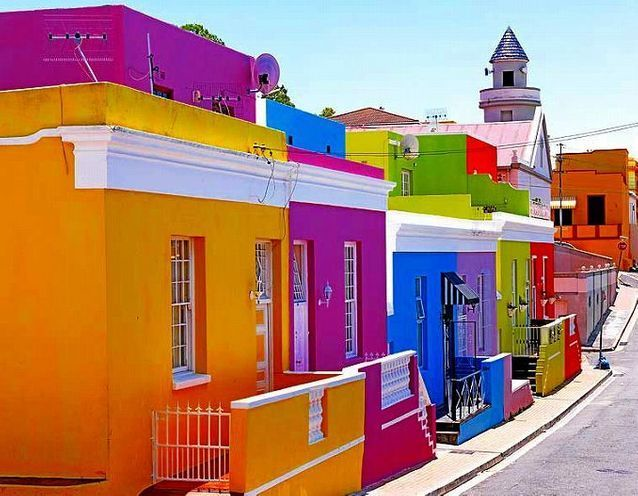
\includegraphics[width=4cm]{ressources/maisons-colorees.png}
             &
            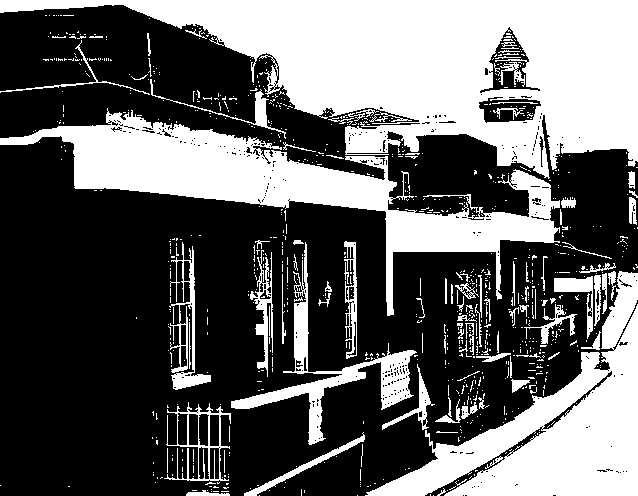
\includegraphics[width=4cm]{ressources/maisons-colorees-NB.png}
            \\
        \end{tabular}
        \captionof{figure}{Modifier le rendu d'une image}
    \end{center}

\end{frame}
\begin{frame}
    \frametitle{}

    \begin{framed}
        \centering Comment élaborer un programme informatique?
    \end{framed}

\end{frame}
\section{Déterminer les étapes: l'algorithme}
\subsection{Découper en étapes simples}
\begin{frame}
    \frametitle{Découper en étapes simples}

    \begin{aretenir}[]
        Pour faire exécuter une tâche à la machine, il faut lui détailler toutes les étapes à réaliser.
    \end{aretenir}

\end{frame}
\begin{frame}
    \frametitle{}

    Pour transformer l'image en noir et blanc, il faut:
    \begin{itemize}
        \item \textbf{Première étape:} Stocker l'image en mémoire.
        \item \textbf{Deuxième étape:} Modifier chaque pixel.
        \item \textbf{Troisième étape:} Enregistrer la nouvelle image.
    \end{itemize}

\end{frame}
\subsection{Détailler les étapes critiques}

\begin{frame}
    \frametitle{Détailler les étapes critiques}

    Une image est une grille composée de pixels. Pour transformer l'image couleur, en noir et blanc, il faut effectuer une opération sur chaque pixel.
    \begin{center}
        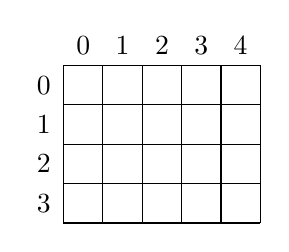
\begin{tikzpicture}[scale=0.5]
            \draw (0,0) grid (5,4);

            \foreach \i in {0,1,2,3}{
                    \node at(-0.5,3.5-\i) {\i};
                }
            \foreach \i in {0,1,2,3,4}{
                    \node at(0.5+\i,4.5) {\i};
                }
        \end{tikzpicture}
        \captionof{figure}{Coordonnées d'un pixel}
        \label{matrice}
    \end{center}

\end{frame}
\begin{frame}
    \frametitle{}

    \textbf{Deuxième étape:} Modifier chaque pixel.
    \begin{center}
        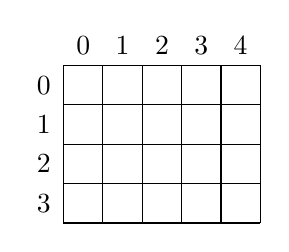
\begin{tikzpicture}[scale=0.5]
            \draw (0,0) grid (5,4);

            \foreach \i in {0,1,2,3}{
                    \node at(-0.5,3.5-\i) {\i};
                }
            \foreach \i in {0,1,2,3,4}{
                    \node at(0.5+\i,4.5) {\i};
                }
        \end{tikzpicture}
        \captionof{figure}{Coordonnées d'un pixel}
        \label{matrice}
    \end{center}
    \begin{itemize}
        \item Parcourir la grille ligne par ligne.
              \begin{itemize}
                  \item Parcourir la ligne colonne par colonne.
                        \begin{itemize}
                            \item Récupérer les couleurs du pixel.
                            \item Le transformer en noir et blanc.
                        \end{itemize}
              \end{itemize}
    \end{itemize}

\end{frame}
\subsection{Traduire l'algorithme: le programme}
\begin{frame}
    \frametitle{Traduire l'algorithme: le programme}

    \begin{aretenir}[]
        Pour que l'ordinateur puisse exécuter l'algorithme, il faut le traduire dans un langage qu'il comprend.
    \end{aretenir}

\end{frame}
\begin{frame}
    \frametitle{}

    \begin{activite}
        \begin{enumerate}
            \item Télécharger le dossier compressé \emph{traitement-image.zip} sur le site \url{https://cviroulaud.github.io} .
            \item Extraire le dossier traitement-image.
            \item Ouvrir le logiciel \emph{Spyder}.
            \item Depuis le logiciel ouvrir le fichier \texttt{\textbf{noir-blanc.py}}.
            \item Observer le programme et repérer les trois étapes de l'algorithme.
        \end{enumerate}
    \end{activite}

\end{frame}
\begin{frame}[fragile]
    \frametitle{Correction}

    \begin{center}
        \begin{lstlisting}[language=Python , basicstyle=\ttfamily\small, xleftmargin=1em, xrightmargin=1em]
from PIL import Image
mon_image = Image.open("maisons-colorees.bmp")
colonne, ligne = mon_image.size
\end{lstlisting}
        \captionof{code}{Stocker l'image}
        \label{CODE}
    \end{center}

\end{frame}
\begin{frame}[fragile]
    \frametitle{}

    \begin{center}
        \begin{lstlisting}[language=Python , basicstyle=\ttfamily\small, xleftmargin=1em, xrightmargin=1em]
for y in range(ligne):
    for x in range(colonne):
        pixel = mon_image.getpixel((x,y))

        moyenne = (pixel[0] + pixel[1] + pixel[2]) // 3
        if moyenne < 128:
            # le pixel sera noir
            r = 0
            v = 0
            b = 0
        else:
            # le pixel sera blanc
            r = 255
            v = 255
            b = 255

        mon_image.putpixel((x,y), (r,v,b))
\end{lstlisting}
        \captionof{code}{Modifier les pixels}
        \label{CODE}
    \end{center}

\end{frame}
\begin{frame}[fragile]
    \frametitle{}

    \begin{center}
        \begin{lstlisting}[language=Python , basicstyle=\ttfamily\small, xleftmargin=1em, xrightmargin=1em]
mon_image.save("maisons-colorees-NB.bmp")
mon_image.show()
\end{lstlisting}
        \captionof{code}{Enregistrer l'image}
        \label{CODE}
    \end{center}

\end{frame}
\begin{frame}
    \frametitle{}

    \begin{activite}
        \begin{enumerate}
            \item Que représente \textbf{\texttt{pixel[0]}}?
            \item Comment fait-on le choix de transformer le pixel en noir ou blanc?
            \item Exécuter le programme.
            \item Modifier le programme pour que l'image obtenue soit plus sombre. Recommencer pour qu'elle soit plus claire.
        \end{enumerate}
    \end{activite}

\end{frame}
\begin{frame}
    \frametitle{Correction}

    
\begin{itemize}
    \item \textbf{\texttt{pixel[0]}} niveau de rouge
    \item \textbf{\texttt{pixel[1]}} niveau de vert
    \item \textbf{\texttt{pixel[2]}} niveau de bleu
\end{itemize}
\end{frame}
\begin{frame}[fragile]
    \frametitle{}

    \begin{center}
        \begin{lstlisting}[language=Python , basicstyle=\ttfamily\small, xleftmargin=1em, xrightmargin=1em]
moyenne = (pixel[0] + pixel[1] + pixel[2]) // 3
# si la moyenne des couleurs RVB est inférieure à un seuil
if moyenne < 128:
    # le pixel sera noir
    r = 0
    v = 0
    b = 0
else:
    # le pixel sera blanc
    r = 255
    v = 255
    b = 255
\end{lstlisting}
        \captionof{code}{Choix de la couleur}
        \label{CODE}
    \end{center}

\end{frame}
\begin{frame}[fragile]
    \frametitle{Correction}

    \begin{center}
        \begin{lstlisting}[language=Python , basicstyle=\ttfamily\small, xleftmargin=1em, xrightmargin=1em]
moyenne = (pixel[0] + pixel[1] + pixel[2]) // 3
# si la moyenne des couleurs RVB est inférieure à un seuil
if moyenne < 200:
    # le pixel sera noir
    r = 0
    v = 0
    b = 0
else:
    # le pixel sera blanc
    r = 255
    v = 255
    b = 255
\end{lstlisting}
        \captionof{code}{Plus sombre: la comparaison est modifiée}
        \label{CODE}
    \end{center}

\end{frame}
\begin{frame}[fragile]
    \frametitle{Correction}

    \begin{center}
        \begin{lstlisting}[language=Python , basicstyle=\ttfamily\small, xleftmargin=1em, xrightmargin=1em]
moyenne = (pixel[0] + pixel[1] + pixel[2]) // 3
# si la moyenne des couleurs RVB est inférieure à un seuil
if moyenne < 50:
    # le pixel sera noir
    r = 0
    v = 0
    b = 0
else:
    # le pixel sera blanc
    r = 255
    v = 255
    b = 255
\end{lstlisting}
        \captionof{code}{Plus clair}
        \label{CODE}
    \end{center}

\end{frame}
\section{Créer d'autres algorithmes}
\begin{frame}
    \frametitle{Créer d'autres algorithmes}

    À partir de l'algorithme de base, nous pouvons imaginer d'autres traitements pour la photographie.

\end{frame}
\begin{frame}
    \frametitle{}

    \begin{activite}
        \begin{enumerate}
            \item Dans les cours précédents, retrouver comment obtenir la couleur grise.
            \item Enregistrer le programme précédent sous le nom \texttt{\textbf{niveaux-gris.py}}.
            \item Modifier le programme pour que l'image obtenue soit en nuances de gris.
            \item Enregistrer le programme précédent sous le nom \texttt{\textbf{niveaux-rouge.py}}.
            \item Modifier le programme pour que l'image obtenue ne contienne que les composantes rouges de chaque pixel.
        \end{enumerate}
    \end{activite}

\end{frame}
\begin{frame}[fragile]
    \frametitle{Correction}

\begin{center}
\begin{lstlisting}[language=Python , basicstyle=\ttfamily\small, xleftmargin=1em, xrightmargin=1em]
for y in range(ligne):
    for x in range(colonne):
        # récupérer le pixel
        pixel = mon_image.getpixel((x,y))

        moyenne = (pixel[0] + pixel[1] + pixel[2]) // 3

        # on replace le nouveau pixel
        mon_image.putpixel((x,y), (moyenne, moyenne, moyenne))
\end{lstlisting}
\captionof{code}{Niveaux de gris}
\label{CODE}
\end{center}

\end{frame}
\begin{frame}[fragile]
    \frametitle{Correction}

\begin{center}
\begin{lstlisting}[language=Python , basicstyle=\ttfamily\small, xleftmargin=1em, xrightmargin=1em]
for y in range(ligne):
    for x in range(colonne):
        # récupérer le pixel
        pixel = mon_image.getpixel((x,y))

        # on replace le nouveau pixel
        mon_image.putpixel((x,y), (pixel[0], 0, 0))
\end{lstlisting}
\captionof{code}{Niveaux de rouge}
\label{CODE}
\end{center}

\end{frame}
\end{document}